\documentclass[aspectratio=169]{beamer}
\usepackage[utf8]{inputenc}
\usepackage[T5]{fontenc}
\usepackage[vietnamese]{babel}
\usepackage{graphicx}
\usepackage{booktabs}
\usepackage{hyperref}
\usepackage{xcolor}
\usepackage{tabularx}

% Cấu hình giao diện Beamer
\usetheme{Madrid}
\usecolortheme{default}
\setbeamertemplate{navigation symbols}{}
\setbeamertemplate{footline}[frame number]

\title[TTNT trong Kế toán - Buổi 7]{Trí tuệ Nhân tạo Ứng dụng trong Kế toán}
\subtitle{Buổi 7: AI trong Tự động hóa Kiểm soát Nội bộ \& Phát hiện Gian lận}
\author{Giảng viên: [Tên Giảng Viên]}
\institute{Đại học Đông Á}
\date{\today}

\begin{document}

\begin{frame}
    \titlepage
\end{frame}

\begin{frame}{Nội dung Bài học}
    \tableofcontents
\end{frame}

% ==========================================
% SECTION 1: Định hình Kế toán & Lượng hóa Môi trường Kiểm soát
% ==========================================
\section{Định hình Kế toán \& Lượng hóa Môi trường Kiểm soát}

\begin{frame}{Sự Sụp đổ của Thomas Cook \& Lỗ hổng Kiểm toán}
    \textbf{Tình huống thực tế:}
    \begin{itemize}
        \item Tập đoàn du lịch khổng lồ Thomas Cook sụp đổ năm 2019.
        \item Các công ty kiểm toán hàng đầu (PwC, EY) liên tục đưa ra báo cáo kiểm toán "sạch" (Clean Audit Reports) trước khi công ty phá sản.
        \item \textbf{Cáo buộc:} Kỳ vọng của thị trường cao hơn yêu cầu quy định. Kiểm toán viên không chỉ xác nhận số liệu quản lý, mà còn phải đánh giá sự bền vững của hệ thống kiểm soát nội bộ.
    \end{itemize}
\end{frame}

\begin{frame}{Khủng hoảng của Kế toán Truyền thống}
    \begin{alertblock}{Điểm giới hạn}
        Liệu kiểm toán viên có thể phát hiện ra những điểm yếu trọng yếu (Material Weaknesses) ngay cả trước khi kiểm toán bắt đầu không?
    \end{alertblock}
    \vspace{0.2cm}
    \begin{itemize}
        \item Các cuộc kiểm toán định kỳ hiện tại không đủ sức đối phó với tốc độ và quy mô dữ liệu khổng lồ.
        \item Kế toán ghi chép những con số khô khan trong quá khứ không còn đủ sức bảo vệ doanh nghiệp.
    \end{itemize}
\end{frame}

\begin{frame}{Định hình lại: Hệ thống Phòng thủ Chủ động}
    \begin{itemize}
        \item Sự trỗi dậy của AI không cướp đi việc làm của kế toán, mà nó \textbf{trao cho chuyên gia những siêu năng lực}.
        \item Công nghệ cày xới hàng núi dữ liệu, tìm kiếm bất thường. Con người (Kế toán viên) chốt hạ quyết định.
        \item Chúng ta chuyển từ việc kiểm tra xác suất kiểu truyền thống sang \textbf{kiểm tra toàn diện 100\%} dựa trên tính toán không mệt mỏi của máy móc.
    \end{itemize}
\end{frame}

\begin{frame}{Ẩn dụ: Phim Minority Report}
    \begin{exampleblock}{Đánh hơi tội phạm trước khi chúng ra tay}
        Hãy tưởng tượng một thuật toán AI có thể phát hiện sự gian lận \textbf{trước khi} cú click chuột cuối cùng phê duyệt chuyển tiền được thực hiện!
    \end{exampleblock}
    \vspace{0.3cm}
    Sự lột xác của kế toán: Dùng Trí tuệ nhân tạo (AI) để đọc vị tâm lý, đánh giá đạo đức và giăng bẫy những thủ đoạn tinh vi nhất.
\end{frame}

\begin{frame}{Rủi ro Tiềm tàng vs Rủi ro Kiểm soát}
    \begin{itemize}
        \item \textbf{Rủi ro tiềm tàng (Inherent Risk):} Rủi ro gắn liền với mô hình kinh doanh, chiến lược của công ty ngay cả khi không có kiểm soát nội bộ (VD: Ngành khai khoáng luôn tiềm ẩn rủi ro môi trường).
        \item \textbf{Rủi ro kiểm soát nội bộ (Internal Control Risk):} Là hậu quả từ hành động của Ban quản lý. Xảy ra khi công ty không có các biện pháp kiểm soát phù hợp (Cố ý lẩn tránh, vô hiệu hóa quy tắc để tham ô).
    \end{itemize}
\end{frame}

\begin{frame}{Nhắc lại Khung COSO (5 Thành phần)}
    Để đánh bại gian lận, chúng ta cần củng cố lõi của Kiểm soát Nội bộ - \textbf{Khung COSO}:
    \begin{enumerate}
        \item Môi trường kiểm soát (Control Environment).
        \item Đánh giá rủi ro (Risk Assessment).
        \item Hoạt động kiểm soát (Control Activities).
        \item Thông tin và Truyền thông (Information \& Communication).
        \item Giám sát (Monitoring).
    \end{enumerate}
\end{frame}

\begin{frame}{Tại sao "Môi trường kiểm soát" lại khó đánh giá?}
    \begin{itemize}
        \item \textbf{Môi trường kiểm soát} chính là "Văn hóa doanh nghiệp" và "Tính chính trực của Ban lãnh đạo" (Tone at the top).
        \item Bài toán khó: Làm sao đưa ra một con số định lượng toán học chính xác cho một thứ trừu tượng như "Đạo đức"?
    \end{itemize}
\end{frame}

\begin{frame}{Bất cập của Phiếu Khảo sát (Surveys)}
    \begin{alertblock}{Văn hóa báo cáo láo}
        Phương pháp cũ dùng phiếu khảo sát hoặc phỏng vấn nhân sự. Nhưng nhược điểm chí mạng là con người luôn có xu hướng \textbf{trả lời những gì cấp trên muốn nghe}. Họ chỉ đánh dấu tích vào ô hoàn hảo cho xong chuyện!
    \end{alertblock}
\end{frame}

\begin{frame}{Ứng dụng AI để "Đo lường Vô hình"}
    \textbf{Giải pháp của kỷ nguyên số:}
    \begin{itemize}
        \item Dùng Trí tuệ Nhân tạo để phân tích cảm xúc và luồng giao tiếp nội bộ trong thời gian thực.
        \item Quét toàn bộ: Hàng ngàn email, biên bản họp hội đồng, tin nhắn Slack, đánh giá ẩn danh trên Glassdoor.
    \end{itemize}
\end{frame}

\begin{frame}{Xử lý Ngôn ngữ Tự nhiên (NLP) vào cuộc}
    \begin{itemize}
        \item \textbf{NLP (Natural Language Processing):} Cho phép máy tính đọc, hiểu và trích xuất ý nghĩa sâu xa từ văn bản phi cấu trúc.
        \item NLP không tìm lỗi sai chính tả. Nó tìm kiếm \textbf{sự thay đổi thái độ} và \textbf{áp lực ngầm}.
    \end{itemize}
\end{frame}

\begin{frame}{NLP đếm trọng số từ vựng (Thuật toán TF-IDF)}
    \begin{itemize}
        \item \textbf{Thuật toán TF-IDF:} Đánh giá tầm quan trọng của một từ vựng trong toàn bộ ngữ cảnh.
        \item Nó không chỉ đếm số lần một từ xuất hiện, mà so sánh nó với văn phong chung của toàn bộ nhân viên.
        \item Nhờ đó, AI có thể nhận diện ngay cả những lời sáo rỗng hoặc những mệnh lệnh bất thường ẩn sau vỏ bọc chuyên nghiệp.
    \end{itemize}
\end{frame}

\begin{frame}{Nhận diện Phong cách Quản lý (Độc đoán vs Hợp tác)}
    \begin{exampleblock}{Môi trường Hợp tác}
        Dùng các cụm từ: \textit{"Giải pháp chung", "Hãy cùng xem xét lại", "Anh cần hỗ trợ gì không?"}
    \end{exampleblock}
    \vspace{0.2cm}
    \begin{alertblock}{Môi trường Độc đoán (Dấu hiệu ép buộc)}
        Liên tục dùng cụm từ: \textit{"Phải xong bằng mọi giá", "Tuyệt mật", "Tôi không cần biết lý do!"}
    \end{alertblock}
    $\Rightarrow$ Thuật toán gán trọng số Rủi ro Cao cho các phòng ban có lối hành xử độc đoán.
\end{frame}

\begin{frame}{Ví dụ: Máy đo nhiệt độ Đạo đức qua Email}
    \begin{itemize}
        \item Việc dùng NLP quét giao tiếp nội bộ giống như doanh nghiệp đang gắn một \textbf{"Chiếc nhiệt kế Đạo đức tự động"} chạy ngầm.
        \item Nó đo được chính xác sức nóng của áp lực công việc mà không cần phát ra tờ phiếu khảo sát nào.
        \item Ngôn từ mà nhân viên dùng vào lúc \textbf{10 giờ đêm khi chạy deadline} chính là dữ liệu chân thực nhất!
    \end{itemize}
\end{frame}

\begin{frame}{Tương quan giữa Nhân sự \& Hệ thống AI}
    \begin{itemize}
        \item Hồ sơ Nhân sự (HR files) và quá trình đào tạo bổ sung thêm dữ liệu cho AI.
        \item Xác định xem bộ phận tuyển dụng có thực sự quan tâm đến "Phân chia nhiệm vụ" (Separation of duties) khi tuyển dụng nhân tài để giảm thiểu rủi ro hay không.
    \end{itemize}
\end{frame}


% ==========================================
% SECTION 2: Khai phá Quy trình & Cái bóng Kỹ thuật số
% ==========================================
\section{Khai phá Quy trình (Process Mining) \& Cái bóng Kỹ thuật số}

\begin{frame}{Hoạt động Kiểm soát \& Khai phá Quy trình}
    \begin{itemize}
        \item Nếu "Môi trường kiểm soát" tạo ra luật chơi, thì "Hoạt động kiểm soát" (Control Activities) là quá trình \textbf{giám sát hành vi thực tế} để tuân thủ luật đó.
        \item Công nghệ lõi hiện nay: \textbf{Khai phá Quy trình (Process Mining)}.
    \end{itemize}
\end{frame}

\begin{frame}{Data-Centric vs Metadata-Centric}
    \begin{table}[]
        \centering
        \begin{tabularx}{\textwidth}{|l|X|X|}
        \hline
        \textbf{Phân loại} & \textbf{Kiểm toán truyền thống (Data-centric)} & \textbf{Process Mining (Metadata-centric)} \\ \hline
        \textbf{Góc nhìn} & Tập trung vào Dữ liệu Giao dịch. & Tập trung vào Siêu dữ liệu (Metadata). \\ \hline
        \textbf{Câu hỏi} & Hóa đơn này trị giá bao nhiêu tiền? Giao dịch với ai? & Giao dịch đó để lại \textbf{cái bóng} gì trên hệ thống? \\ \hline
        \textbf{Kết quả} & Tìm kiếm số tiền bị thất thoát. & Phát hiện lỗ hổng quy trình vận hành. \\ \hline
        \end{tabularx}
    \end{table}
\end{frame}

\begin{frame}{Cái bóng Kỹ thuật số (Digital Shadow) là gì?}
    \textbf{Siêu dữ liệu (Metadata) - Nhật ký sự kiện (Event Logs):}
    \begin{itemize}
        \item Ai đã truy cập vào hệ thống?
        \item Đăng nhập từ địa chỉ IP nào?
        \item Thao tác đó được thực hiện vào mấy giờ, mấy phút (tính đến từng giây)?
        \item Process Mining gom hàng triệu dấu vết nhỏ này để tái tạo \textbf{toàn bộ đường đi thực tế} của dữ liệu!
    \end{itemize}
\end{frame}

\begin{frame}{Đánh giá Kiểm soát Nội bộ Tự động (Hình 9.1)}
    \begin{figure}
        \centering
        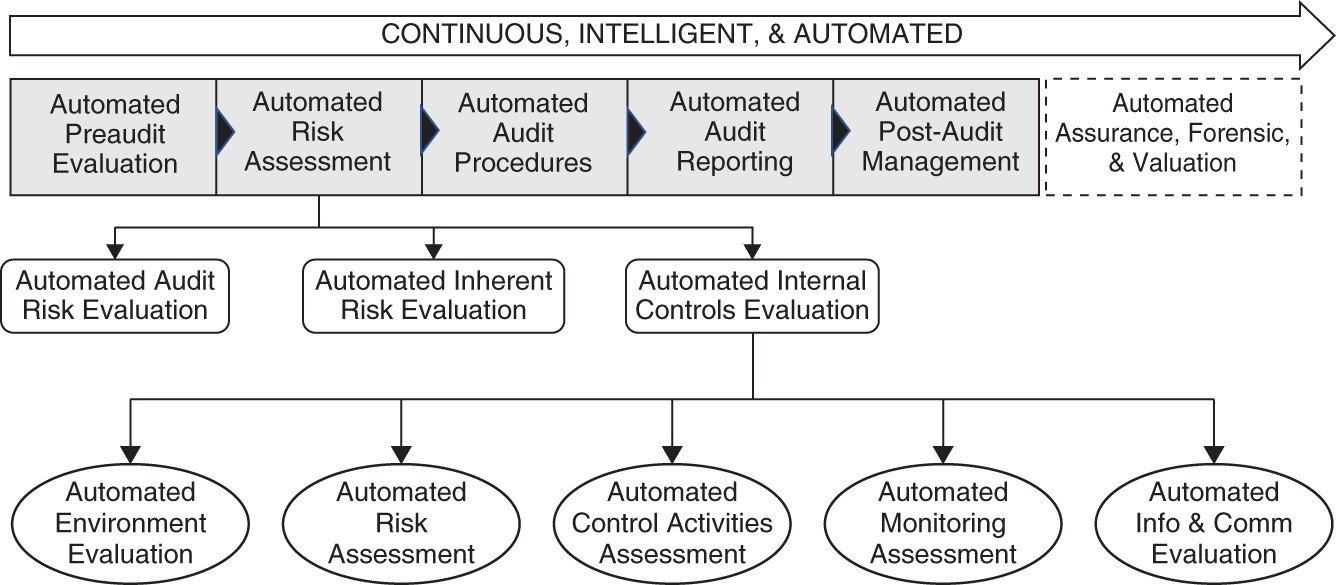
\includegraphics[height=0.65\textheight]{../../Figures/Buoi_07A/FIGURE 9.1 Automation of Internal Controls Evaluation.jpeg}
        \caption{Mô hình Đánh giá Kiểm soát Nội bộ Tự động (COSO)}
    \end{figure}
\end{frame}

\begin{frame}{Bất kiêm nhiệm (Segregation of Duties) trong Lý thuyết}
    \begin{exampleblock}{Quy tắc Kinh điển để Chống Tham ô}
        Nhân viên tạo một nhà cung cấp mới (Vendor) và người phê duyệt chuyển tiền cho nhà cung cấp đó \textbf{phải là hai người hoàn toàn khác nhau}.
    \end{exampleblock}
\end{frame}

\begin{frame}{Bất kiêm nhiệm trên Thực tế (Cách lách luật)}
    \begin{itemize}
        \item Kẻ gian (một Kế toán trưởng) muốn tham ô, họ mượn tài khoản của cấp dưới để tự tạo "Nhà cung cấp ma".
        \item Sau đó dùng tài khoản của chính mình để Duyệt thanh toán cho "Nhà cung cấp ma" đó.
        \item Trên sổ sách (Data-centric): Giao dịch hoàn toàn hợp lệ, đủ 2 chữ ký điện tử, có đủ hóa đơn. Kiểm toán truyền thống sẽ bị qua mặt!
    \end{itemize}
\end{frame}

\begin{frame}{Case Study: 6 Phút của Gian lận}
    \begin{alertblock}{Đòn giáng của Process Mining}
        Thuật toán không quan tâm tờ hóa đơn. Nó quét Nhật ký hệ thống và nhận ra: 
        Tài khoản Nhân viên A tạo vendor lúc \textbf{09:12 AM từ Địa chỉ IP 192.168.1.40}. 
        Chỉ đúng \textbf{6 phút sau}, tài khoản Giám đốc B phê duyệt chuyển tiền từ \textbf{chính Địa chỉ IP 192.168.1.40} đó!
    \end{alertblock}
    $\Rightarrow$ Cùng một máy tính, thực hiện 2 thao tác đối lập trong 6 phút. Cờ đỏ báo động ngay lập tức!
\end{frame}

\begin{frame}{Bài toán Cảnh báo giả (False Positives)}
    \begin{itemize}
        \item Mọi cái click chuột, mọi lần đăng nhập muộn đều bị ghi lại. 
        \item Nếu hệ thống Process Mining nguyên thủy cảnh báo bất cứ lúc nào có đăng nhập vào 2h sáng, nó sẽ tạo ra một \textbf{núi rác cảnh báo}.
        \item Kế toán viên sẽ kiệt sức vì những tiếng báo động giả (Alert Fatigue).
    \end{itemize}
\end{frame}

\begin{frame}{Cảnh báo giả: Khóa sổ lúc 2h sáng hay Gian lận?}
    \begin{itemize}
        \item \textbf{Trường hợp 1:} Kế toán đăng nhập 2h sáng ngày 30/12 để làm quyết toán khóa sổ cuối năm. $\Rightarrow$ \textbf{Hợp lý.}
        \item \textbf{Trường hợp 2:} Kế toán đăng nhập 2h sáng ngày 14/03 để thay đổi Số tài khoản ngân hàng của một nhà cung cấp lớn. $\Rightarrow$ \textbf{Có mùi gian lận!}
    \end{itemize}
\end{frame}

\begin{frame}{Giải pháp: Process Mining + Machine Learning}
    \begin{itemize}
        \item Dùng Machine Learning (Học máy) để hệ thống \textbf{tự học bớt ngu ngơ đi}.
        \item Cần sự can thiệp của Kế toán viên lão luyện (Human-in-the-loop). 
        \item Chuyên gia sẽ "dán nhãn" cho AI: Dạy nó phân biệt đâu là áp lực khóa sổ bình thường, đâu là hành vi đánh cắp tài sản.
    \end{itemize}
\end{frame}

\begin{frame}{Đánh giá Môi trường Kiểm soát Tự động (Hình 9.2)}
    \begin{figure}
        \centering
        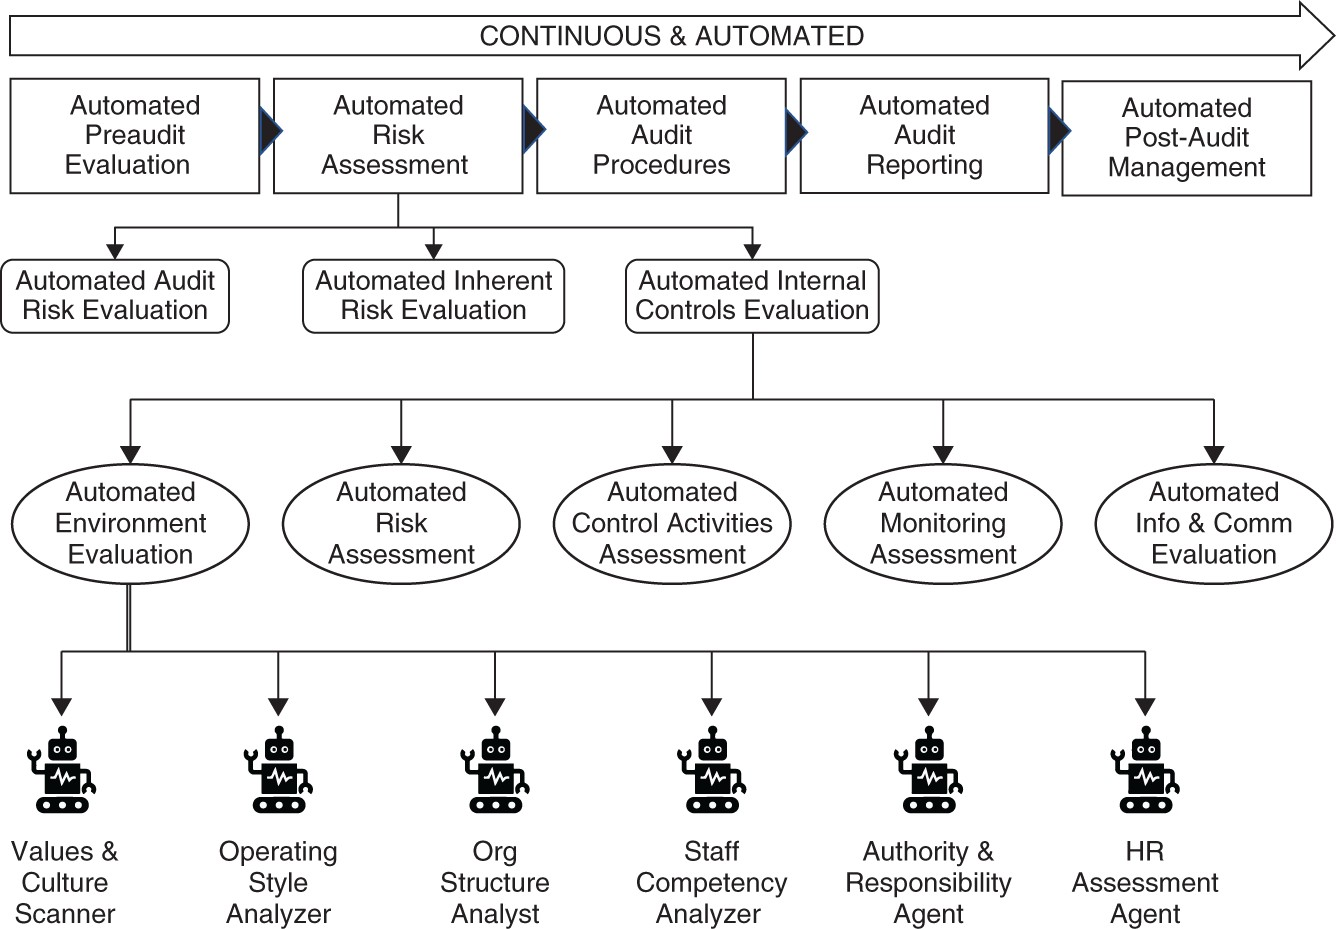
\includegraphics[height=0.65\textheight]{../../Figures/Buoi_07A/FIGURE 9.2 Automated Environment Evaluation.jpeg}
        \caption{Đánh giá Môi trường Kiểm soát Tự động}
    \end{figure}
\end{frame}


% ==========================================
% SECTION 3: Kim cương Gian lận, Clustering & Rủi ro AI
% ==========================================
\section{Kim cương Gian lận, Clustering \& Rủi ro AI}

\begin{frame}{Cây Gian lận (Fraud Tree của ACFE)}
    Dù công nghệ tối tân đến đâu, gian lận vẫn xảy ra vì đó là bản chất con người. Để AI bắt được kẻ gian, nó phải hiểu hình hài của chúng:
    \begin{enumerate}
        \item Tham nhũng (Corruption)
        \item Chiếm đoạt tài sản (Asset Misappropriation)
        \item Gian lận Báo cáo Tài chính (Financial Statement Fraud)
    \end{enumerate}
\end{frame}

\begin{frame}{Tam giác Gian lận vs Kim cương Gian lận}
    \begin{itemize}
        \item \textbf{Tam giác gian lận truyền thống (Cressey):} Áp lực (Pressure), Cơ hội (Opportunity), Biện minh (Rationalization).
        \item \textbf{Kim cương gian lận (Fraud Diamond - Wolfe \& Hermanson):} Trong doanh nghiệp hiện đại, 3 yếu tố trên là chưa đủ. Yếu tố thứ 4 quyết định tất cả chính là \textbf{Năng lực (Capability)}.
    \end{itemize}
\end{frame}

\begin{frame}{Phép ví von: Gian lận như một vụ cháy nổ}
    Hãy hình dung Kim cương gian lận chính là công thức tạo nên một vụ cháy nổ:
    \begin{itemize}
        \item \textbf{Áp lực:} Là "Chất đốt" (Nợ nần, thiếu tiền).
        \item \textbf{Cơ hội:} Là không gian đầy "Oxy" (Lỗ hổng hệ thống).
        \item \textbf{Biện minh:} Là "Nhiệt độ môi trường" (Tự nhủ: "Mình chỉ mượn tạm thôi").
    \end{itemize}
    \textit{Ba yếu tố trên tạo ra một căn phòng cực kỳ dễ nổ. Nhưng để vụ nổ thực sự xảy ra...}
\end{frame}

\begin{frame}{Góc Năng lực (Capability): Mồi lửa châm ngòi}
    \begin{itemize}
        \item \textbf{Năng lực (Capability):} Chính là "Mồi lửa châm ngòi".
        \item Kẻ đó phải đủ khôn ngoan, hiểu rõ ngóc ngách của hệ thống để biết mình có thể qua mặt được cả công ty. Thường là những Quản lý cấp cao.
    \end{itemize}
\end{frame}

\begin{frame}{Dùng AI để dập tắt "Nhiệt độ" (Biện minh)}
    \begin{itemize}
        \item \textbf{Góc Cơ hội:} Đã bị Process Mining đánh thẳng vào, chặn đứng lỗ hổng.
        \item \textbf{Góc Biện minh \& Năng lực:} Dùng NLP để phân tích hợp đồng, báo cáo, giọng điệu của Ban giám đốc nhằm tìm ra "ngôn ngữ thao túng".
    \end{itemize}
\end{frame}

\begin{frame}{Quản trị Lợi nhuận (Earnings Management)}
    \begin{exampleblock}{Ranh giới mỏng manh}
        \textbf{Earnings Management} là việc xào xáo số liệu kế toán (linh hoạt ước tính, dồn chi phí) một cách cực kỳ tinh vi để đạt được kỳ vọng của cổ đông mà không bị coi là vi phạm pháp luật công khai.
    \end{exampleblock}
\end{frame}

\begin{frame}{Phát hiện Earnings Management bằng NLP}
    \begin{itemize}
        \item NLP đối chiếu chéo \textbf{Giọng điệu email nội bộ} với \textbf{Báo cáo ra công chúng}.
        \item Nếu trong nội bộ công ty, Sếp đang cuống cuồng, dùng từ ngữ tiêu cực (Chất đốt)...
        \item ...Nhưng trên Báo cáo Tài chính gửi nhà đầu tư lại tự tin ngút ngàn, dùng ngôn từ ngụy tạo che đậy...
        \item Thuật toán sẽ khoanh vùng sự bất đồng bộ này ngay lập tức!
    \end{itemize}
\end{frame}

\begin{frame}{Truy tìm "Unknown Unknowns" với Học Không Giám Sát}
    \begin{alertblock}{Hạn chế của dữ liệu quá khứ}
        Nếu chúng ta chỉ dạy AI tìm gian lận dựa trên dữ liệu quá khứ, nó sẽ bị "mù" trước những thủ đoạn chiếm đoạt hoàn toàn mới mẻ, chưa từng có tiền lệ.
    \end{alertblock}
    $\Rightarrow$ Cần sự can thiệp của \textbf{Học không giám sát (Unsupervised Learning)}.
\end{frame}

\begin{frame}{Phân cụm (Clustering)}
    \begin{itemize}
        \item Không cần con người dán nhãn từ trước. AI được thả vào một biển dữ liệu khổng lồ.
        \item Nó dùng thuật toán Phân cụm (Clustering) để tự động gom các giao dịch giống nhau lại thành khối.
        \item Bất cứ giao dịch nào "chơ vơ" không nằm trong cụm nào sẽ bị lôi ra ánh sáng.
    \end{itemize}
\end{frame}

\begin{frame}{Case Study: Giao dịch 9.999 USD để lách luật}
    \begin{itemize}
        \item Quy tắc công ty: Giao dịch trên 10.000 USD phải có sự phê duyệt của 2 Giám đốc.
        \item Kẻ gian lách luật: Liên tục tạo ra các hóa đơn có giá trị \textbf{9.999 USD} (vừa khít dưới ngưỡng) vào các ngày cuối tuần.
        \item Con người có thể không rảnh để đi tìm mẫu đó. Nhưng AI phân cụm thấy một đống các giao dịch tụ tập quanh mốc 9.999 USD đầy dị thường, toán học không biết nói dối!
    \end{itemize}
\end{frame}

\begin{frame}{Đánh giá Chéo Đa chiều (STOP SCAM)}
    \textbf{Không kết tội ngay, chỉ tính xác suất rủi ro cao:}
    \begin{itemize}
        \item Dữ liệu nhân sự: Một nhân viên vừa bị giáng chức (Áp lực).
        \item Dữ liệu NLP: Email nội bộ chứa đầy từ ngữ tức giận, thù hằn (Biện minh/Thái độ).
        \item AI sẽ tự động thắt chặt quyền truy cập của người này trên hệ thống tài chính để ngăn chặn nguy cơ trả đũa. Tuyến phòng thủ từ xa!
    \end{itemize}
\end{frame}

\begin{frame}{Rủi ro Tương lai: Khi thuật toán bị thao túng}
    \begin{itemize}
        \item Từ đầu đến giờ, chúng ta mặc định AI là "công cụ trung lập" để giám sát con người.
        \item \textbf{Nhưng điều gì xảy ra nếu chính AI bị thao túng?}
        \item Nếu thuật toán được cấu hình mệnh lệnh cao nhất là "Tối ưu hóa lợi nhuận bằng mọi giá"?
    \end{itemize}
\end{frame}

\begin{frame}{Con dao hai lưỡi: Ai sẽ kiểm toán cỗ máy?}
    \begin{itemize}
        \item AI có thể tự động \textbf{che giấu các khoản lỗ} bằng những giao dịch tài chính phái sinh phức tạp (chẻ nhỏ, giao dịch cao tần) mà bộ não con người không thể giải mã nổi!
        \item Trí tuệ nhân tạo là giải pháp ngăn chặn rủi ro tuyệt vời nhất, nhưng cũng chính là \textbf{rủi ro lớn nhất} mà hệ thống kiểm soát nội bộ tương lai phải đối mặt.
    \end{itemize}
\end{frame}

\begin{frame}{Tổng kết Bài học}
    \begin{itemize}
        \item AI đánh giá "Môi trường kiểm soát" bằng cách quét giọng điệu, văn phong nội bộ thay vì dựa vào phiếu khảo sát phiến diện.
        \item Process Mining theo dõi "Cái bóng kỹ thuật số", đập tan chiêu trò lách luật bất kiêm nhiệm.
        \item Học máy phân cụm (Clustering) bắt thóp mọi giao dịch dị thường chưa từng có tiền lệ.
        \item Tương lai: Nghề kiểm toán chuyển từ kiểm toán số liệu sang \textbf{Kiểm toán Thuật toán (Algorithm Auditing)}.
    \end{itemize}
\end{frame}

\begin{frame}
    \centering
    \Huge \textbf{Cảm ơn các bạn đã lắng nghe!}
    
    \vspace{0.5cm}
    \Large Hỏi \& Đáp
\end{frame}

\end{document}
